\section{knowtreemodel Class Reference}
\label{classknowtreemodel}\index{knowtreemodel@{knowtreemodel}}
{\tt \#include $<$knowtreemodel.h$>$}

Inheritance diagram for knowtreemodel:\begin{figure}[H]
\begin{center}
\leavevmode
\includegraphics[width=115pt]{classknowtreemodel__inherit__graph}
\end{center}
\end{figure}
Collaboration diagram for knowtreemodel:\begin{figure}[H]
\begin{center}
\leavevmode
\includegraphics[width=115pt]{classknowtreemodel__coll__graph}
\end{center}
\end{figure}
\subsection*{Public Member Functions}
\begin{CompactItemize}
\item 
{\bf knowtreemodel} (const QString\-List \&headers, QDom\-Document dommodel, QObject $\ast$parent=0)
\item 
{\bf $\sim$knowtreemodel} ()
\item 
QDom\-Element {\bf export\_\-fullmodeldata\_\-to\_\-dom} ({\bf Tree\-Item} $\ast$root)
\item 
void {\bf add\_\-new\_\-child\_\-branch} (const QModel\-Index \&index, QString id, QString name)
\item 
void {\bf add\_\-new\_\-sibling\_\-branch} (const QModel\-Index \&index, QString id, QString name)
\item 
void {\bf add\_\-new\_\-branch} ({\bf Tree\-Item} $\ast$parent, QString id, QString name)
\item 
QModel\-Index {\bf move\_\-up\_\-branch} (const QModel\-Index \&index)
\item 
QModel\-Index {\bf move\_\-dn\_\-branch} (const QModel\-Index \&index)
\item 
QModel\-Index {\bf index\-Children} (const QModel\-Index \&parent, int n) const
\item 
QModel\-Index {\bf get\_\-item\_\-index} ({\bf Tree\-Item} $\ast$item)
\end{CompactItemize}
\subsection*{Private Member Functions}
\begin{CompactItemize}
\item 
void {\bf setup\-Model\-Data} (QDom\-Document dommodel, {\bf Tree\-Item} $\ast$parent)
\item 
void {\bf parsenodeelement} (QDom\-Element n, {\bf Tree\-Item} $\ast$parent)
\item 
void {\bf parsetreetodom} (QDom\-Element $\ast$xmldata, {\bf Tree\-Item} $\ast$curritem)
\item 
QModel\-Index {\bf move\_\-updn\_\-branch} (const QModel\-Index \&index, int direction)
\item 
QModel\-Index {\bf get\_\-item\_\-index\_\-recurse} (QModel\-Index currindex, {\bf Tree\-Item} $\ast$finditem, int mode)
\end{CompactItemize}


\subsection{Detailed Description}




Definition at line 12 of file knowtreemodel.h.

\subsection{Constructor \& Destructor Documentation}
\index{knowtreemodel@{knowtreemodel}!knowtreemodel@{knowtreemodel}}
\index{knowtreemodel@{knowtreemodel}!knowtreemodel@{knowtreemodel}}
\subsubsection{\setlength{\rightskip}{0pt plus 5cm}knowtreemodel::knowtreemodel (const QString\-List \& {\em headers}, QDom\-Document {\em dommodel}, QObject $\ast$ {\em parent} = {\tt 0})}\label{classknowtreemodel_f0739625bf50ab26782b7b18cee9ee49}




Definition at line 13 of file knowtreemodel.cpp.

References Tree\-Model::root\-Item, and setup\-Model\-Data().

Here is the call graph for this function:\begin{figure}[H]
\begin{center}
\leavevmode
\includegraphics[width=223pt]{classknowtreemodel_f0739625bf50ab26782b7b18cee9ee49_cgraph}
\end{center}
\end{figure}
\index{knowtreemodel@{knowtreemodel}!~knowtreemodel@{$\sim$knowtreemodel}}
\index{~knowtreemodel@{$\sim$knowtreemodel}!knowtreemodel@{knowtreemodel}}
\subsubsection{\setlength{\rightskip}{0pt plus 5cm}knowtreemodel::$\sim$knowtreemodel ()}\label{classknowtreemodel_a89ceb62d7b430e72b8e8be5fb195316}




Definition at line 33 of file knowtreemodel.cpp.

References Tree\-Model::root\-Item.

\subsection{Member Function Documentation}
\index{knowtreemodel@{knowtreemodel}!export_fullmodeldata_to_dom@{export\_\-fullmodeldata\_\-to\_\-dom}}
\index{export_fullmodeldata_to_dom@{export\_\-fullmodeldata\_\-to\_\-dom}!knowtreemodel@{knowtreemodel}}
\subsubsection{\setlength{\rightskip}{0pt plus 5cm}QDom\-Element knowtreemodel::export\_\-fullmodeldata\_\-to\_\-dom ({\bf Tree\-Item} $\ast$ {\em root})}\label{classknowtreemodel_a1a1e8307a9a1d6de4432ae8bf28a42d}




Definition at line 99 of file knowtreemodel.cpp.

References parsetreetodom().

Referenced by treescreen::save\_\-knowtree().

Here is the call graph for this function:\begin{figure}[H]
\begin{center}
\leavevmode
\includegraphics[width=259pt]{classknowtreemodel_a1a1e8307a9a1d6de4432ae8bf28a42d_cgraph}
\end{center}
\end{figure}


Here is the caller graph for this function:\begin{figure}[H]
\begin{center}
\leavevmode
\includegraphics[width=351pt]{classknowtreemodel_a1a1e8307a9a1d6de4432ae8bf28a42d_icgraph}
\end{center}
\end{figure}
\index{knowtreemodel@{knowtreemodel}!add_new_child_branch@{add\_\-new\_\-child\_\-branch}}
\index{add_new_child_branch@{add\_\-new\_\-child\_\-branch}!knowtreemodel@{knowtreemodel}}
\subsubsection{\setlength{\rightskip}{0pt plus 5cm}void knowtreemodel::add\_\-new\_\-child\_\-branch (const QModel\-Index \& {\em index}, QString {\em id}, QString {\em name})}\label{classknowtreemodel_9a5cf7df4f0e7a1362e1eaa725b7826b}




Definition at line 175 of file knowtreemodel.cpp.

References add\_\-new\_\-branch(), Tree\-Model::get\-Item(), and Tree\-Model::parent().

Referenced by treescreen::ins\_\-subbranch().

Here is the call graph for this function:\begin{figure}[H]
\begin{center}
\leavevmode
\includegraphics[width=404pt]{classknowtreemodel_9a5cf7df4f0e7a1362e1eaa725b7826b_cgraph}
\end{center}
\end{figure}
\index{knowtreemodel@{knowtreemodel}!add_new_sibling_branch@{add\_\-new\_\-sibling\_\-branch}}
\index{add_new_sibling_branch@{add\_\-new\_\-sibling\_\-branch}!knowtreemodel@{knowtreemodel}}
\subsubsection{\setlength{\rightskip}{0pt plus 5cm}void knowtreemodel::add\_\-new\_\-sibling\_\-branch (const QModel\-Index \& {\em index}, QString {\em id}, QString {\em name})}\label{classknowtreemodel_db22fa31851d2020284c5713ad98e1f1}




Definition at line 187 of file knowtreemodel.cpp.

References add\_\-new\_\-branch(), Tree\-Model::get\-Item(), Tree\-Item::parent(), and Tree\-Model::parent().

Referenced by treescreen::ins\_\-branch().

Here is the call graph for this function:\begin{figure}[H]
\begin{center}
\leavevmode
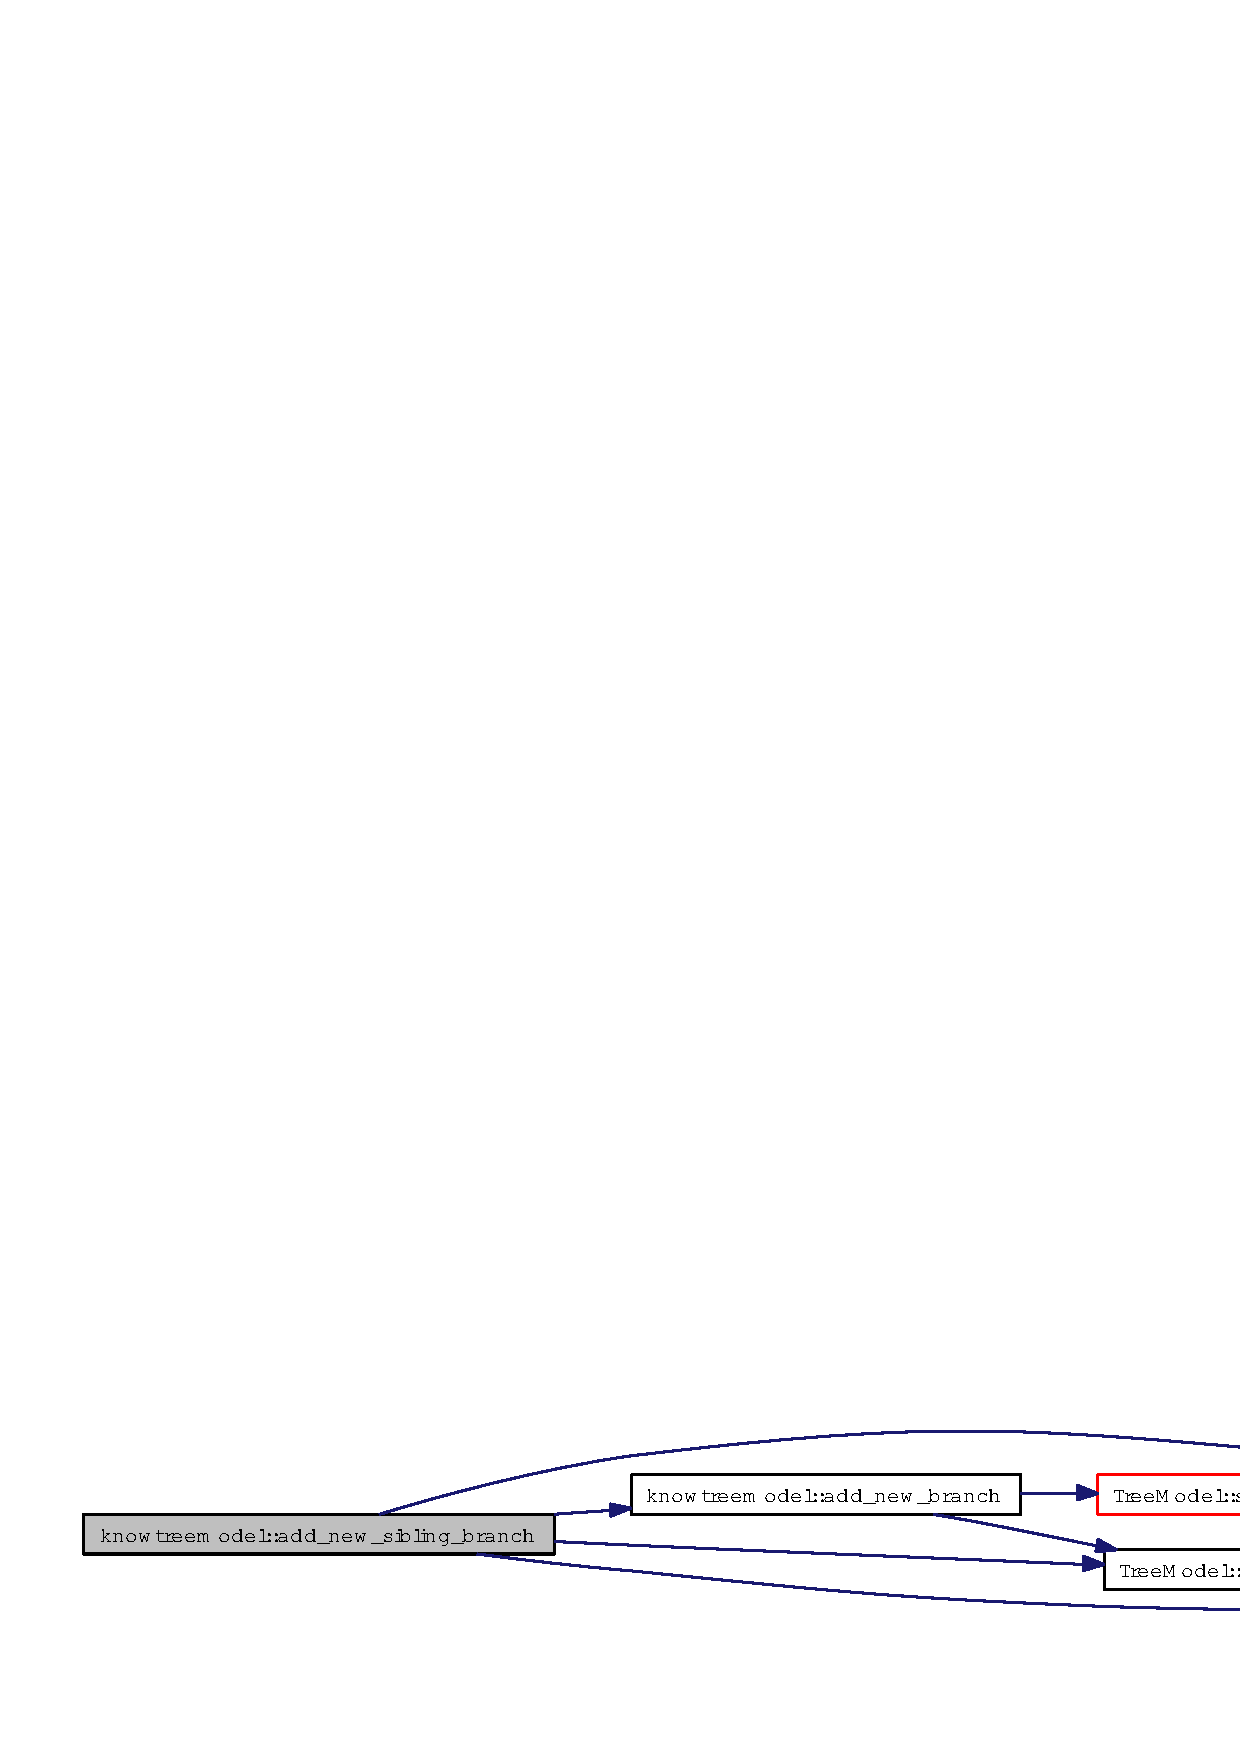
\includegraphics[width=399pt]{classknowtreemodel_db22fa31851d2020284c5713ad98e1f1_cgraph}
\end{center}
\end{figure}
\index{knowtreemodel@{knowtreemodel}!add_new_branch@{add\_\-new\_\-branch}}
\index{add_new_branch@{add\_\-new\_\-branch}!knowtreemodel@{knowtreemodel}}
\subsubsection{\setlength{\rightskip}{0pt plus 5cm}void knowtreemodel::add\_\-new\_\-branch ({\bf Tree\-Item} $\ast$ {\em parent}, QString {\em id}, QString {\em name})}\label{classknowtreemodel_3870358ee6419e354a0e64d35602c496}




Definition at line 200 of file knowtreemodel.cpp.

References Tree\-Model::parent(), and Tree\-Model::set\-Data().

Referenced by add\_\-new\_\-child\_\-branch(), and add\_\-new\_\-sibling\_\-branch().

Here is the call graph for this function:\begin{figure}[H]
\begin{center}
\leavevmode
\includegraphics[width=277pt]{classknowtreemodel_3870358ee6419e354a0e64d35602c496_cgraph}
\end{center}
\end{figure}


Here is the caller graph for this function:\begin{figure}[H]
\begin{center}
\leavevmode
\includegraphics[width=247pt]{classknowtreemodel_3870358ee6419e354a0e64d35602c496_icgraph}
\end{center}
\end{figure}
\index{knowtreemodel@{knowtreemodel}!move_up_branch@{move\_\-up\_\-branch}}
\index{move_up_branch@{move\_\-up\_\-branch}!knowtreemodel@{knowtreemodel}}
\subsubsection{\setlength{\rightskip}{0pt plus 5cm}QModel\-Index knowtreemodel::move\_\-up\_\-branch (const QModel\-Index \& {\em index})}\label{classknowtreemodel_dde544e3e416a51e6e132fa2f07426f8}




Definition at line 215 of file knowtreemodel.cpp.

References move\_\-updn\_\-branch().

Referenced by treescreen::move\_\-updn\_\-branch().

Here is the call graph for this function:\begin{figure}[H]
\begin{center}
\leavevmode
\includegraphics[width=396pt]{classknowtreemodel_dde544e3e416a51e6e132fa2f07426f8_cgraph}
\end{center}
\end{figure}


Here is the caller graph for this function:\begin{figure}[H]
\begin{center}
\leavevmode
\includegraphics[width=223pt]{classknowtreemodel_dde544e3e416a51e6e132fa2f07426f8_icgraph}
\end{center}
\end{figure}
\index{knowtreemodel@{knowtreemodel}!move_dn_branch@{move\_\-dn\_\-branch}}
\index{move_dn_branch@{move\_\-dn\_\-branch}!knowtreemodel@{knowtreemodel}}
\subsubsection{\setlength{\rightskip}{0pt plus 5cm}QModel\-Index knowtreemodel::move\_\-dn\_\-branch (const QModel\-Index \& {\em index})}\label{classknowtreemodel_d9fc7fb894fad944f7e02556ddfa375e}




Definition at line 222 of file knowtreemodel.cpp.

References move\_\-updn\_\-branch().

Referenced by treescreen::move\_\-updn\_\-branch().

Here is the call graph for this function:\begin{figure}[H]
\begin{center}
\leavevmode
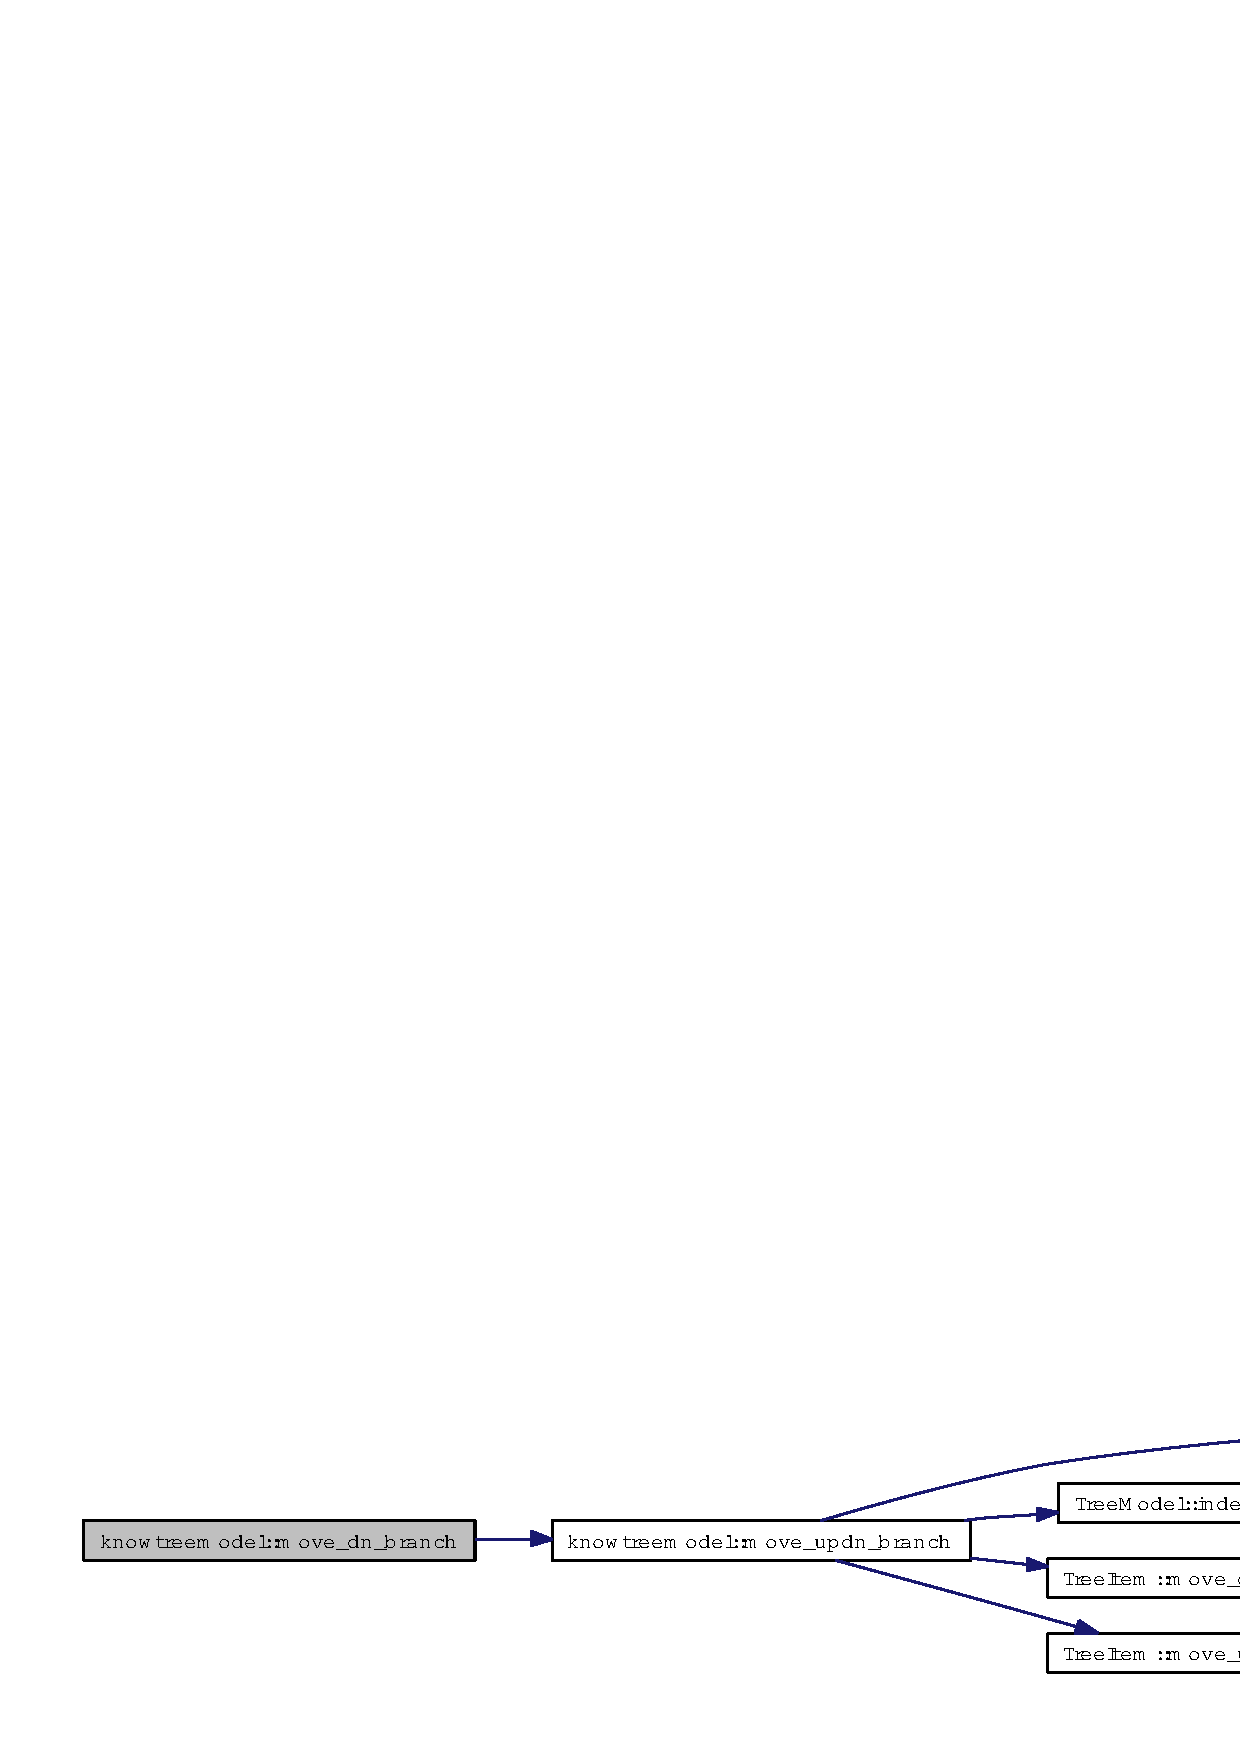
\includegraphics[width=396pt]{classknowtreemodel_d9fc7fb894fad944f7e02556ddfa375e_cgraph}
\end{center}
\end{figure}


Here is the caller graph for this function:\begin{figure}[H]
\begin{center}
\leavevmode
\includegraphics[width=223pt]{classknowtreemodel_d9fc7fb894fad944f7e02556ddfa375e_icgraph}
\end{center}
\end{figure}
\index{knowtreemodel@{knowtreemodel}!indexChildren@{indexChildren}}
\index{indexChildren@{indexChildren}!knowtreemodel@{knowtreemodel}}
\subsubsection{\setlength{\rightskip}{0pt plus 5cm}QModel\-Index knowtreemodel::index\-Children (const QModel\-Index \& {\em parent}, int {\em n}) const}\label{classknowtreemodel_7802e8122c237aabd9050ed36295999f}




Definition at line 270 of file knowtreemodel.cpp.

References Tree\-Item::child(), Tree\-Item::child\-Count(), Tree\-Model::get\-Item(), and Tree\-Model::index().

Referenced by treescreen::ins\_\-subbranch().

Here is the call graph for this function:\begin{figure}[H]
\begin{center}
\leavevmode
\includegraphics[width=264pt]{classknowtreemodel_7802e8122c237aabd9050ed36295999f_cgraph}
\end{center}
\end{figure}
\index{knowtreemodel@{knowtreemodel}!get_item_index@{get\_\-item\_\-index}}
\index{get_item_index@{get\_\-item\_\-index}!knowtreemodel@{knowtreemodel}}
\subsubsection{\setlength{\rightskip}{0pt plus 5cm}QModel\-Index knowtreemodel::get\_\-item\_\-index ({\bf Tree\-Item} $\ast$ {\em item})}\label{classknowtreemodel_6e9e460ebb16f09d1015fcc69ea943e9}




Definition at line 311 of file knowtreemodel.cpp.

References Tree\-Item::child\-Number().

Referenced by mainwindow::set\_\-tree\_\-position().

Here is the call graph for this function:\begin{figure}[H]
\begin{center}
\leavevmode
\includegraphics[width=197pt]{classknowtreemodel_6e9e460ebb16f09d1015fcc69ea943e9_cgraph}
\end{center}
\end{figure}


Here is the caller graph for this function:\begin{figure}[H]
\begin{center}
\leavevmode
\includegraphics[width=371pt]{classknowtreemodel_6e9e460ebb16f09d1015fcc69ea943e9_icgraph}
\end{center}
\end{figure}
\index{knowtreemodel@{knowtreemodel}!setupModelData@{setupModelData}}
\index{setupModelData@{setupModelData}!knowtreemodel@{knowtreemodel}}
\subsubsection{\setlength{\rightskip}{0pt plus 5cm}void knowtreemodel::setup\-Model\-Data (QDom\-Document {\em dommodel}, {\bf Tree\-Item} $\ast$ {\em parent})\hspace{0.3cm}{\tt  [private]}}\label{classknowtreemodel_f68a64ca103c6f21899c87cf3392d011}




Definition at line 40 of file knowtreemodel.cpp.

References Tree\-Model::parent(), and parsenodeelement().

Referenced by knowtreemodel().

Here is the call graph for this function:\begin{figure}[H]
\begin{center}
\leavevmode
\includegraphics[width=305pt]{classknowtreemodel_f68a64ca103c6f21899c87cf3392d011_cgraph}
\end{center}
\end{figure}


Here is the caller graph for this function:\begin{figure}[H]
\begin{center}
\leavevmode
\includegraphics[width=223pt]{classknowtreemodel_f68a64ca103c6f21899c87cf3392d011_icgraph}
\end{center}
\end{figure}
\index{knowtreemodel@{knowtreemodel}!parsenodeelement@{parsenodeelement}}
\index{parsenodeelement@{parsenodeelement}!knowtreemodel@{knowtreemodel}}
\subsubsection{\setlength{\rightskip}{0pt plus 5cm}void knowtreemodel::parsenodeelement (QDom\-Element {\em n}, {\bf Tree\-Item} $\ast$ {\em parent})\hspace{0.3cm}{\tt  [private]}}\label{classknowtreemodel_01a2b1a9a1edc6b25210a27a6cca5a7c}




Definition at line 57 of file knowtreemodel.cpp.

References Tree\-Item::child(), Tree\-Item::child\-Count(), Tree\-Item::insert\-Children(), Tree\-Model::parent(), Tree\-Item::recordtable\_\-init(), and Tree\-Model::set\-Data().

Referenced by setup\-Model\-Data().

Here is the call graph for this function:\begin{figure}[H]
\begin{center}
\leavevmode
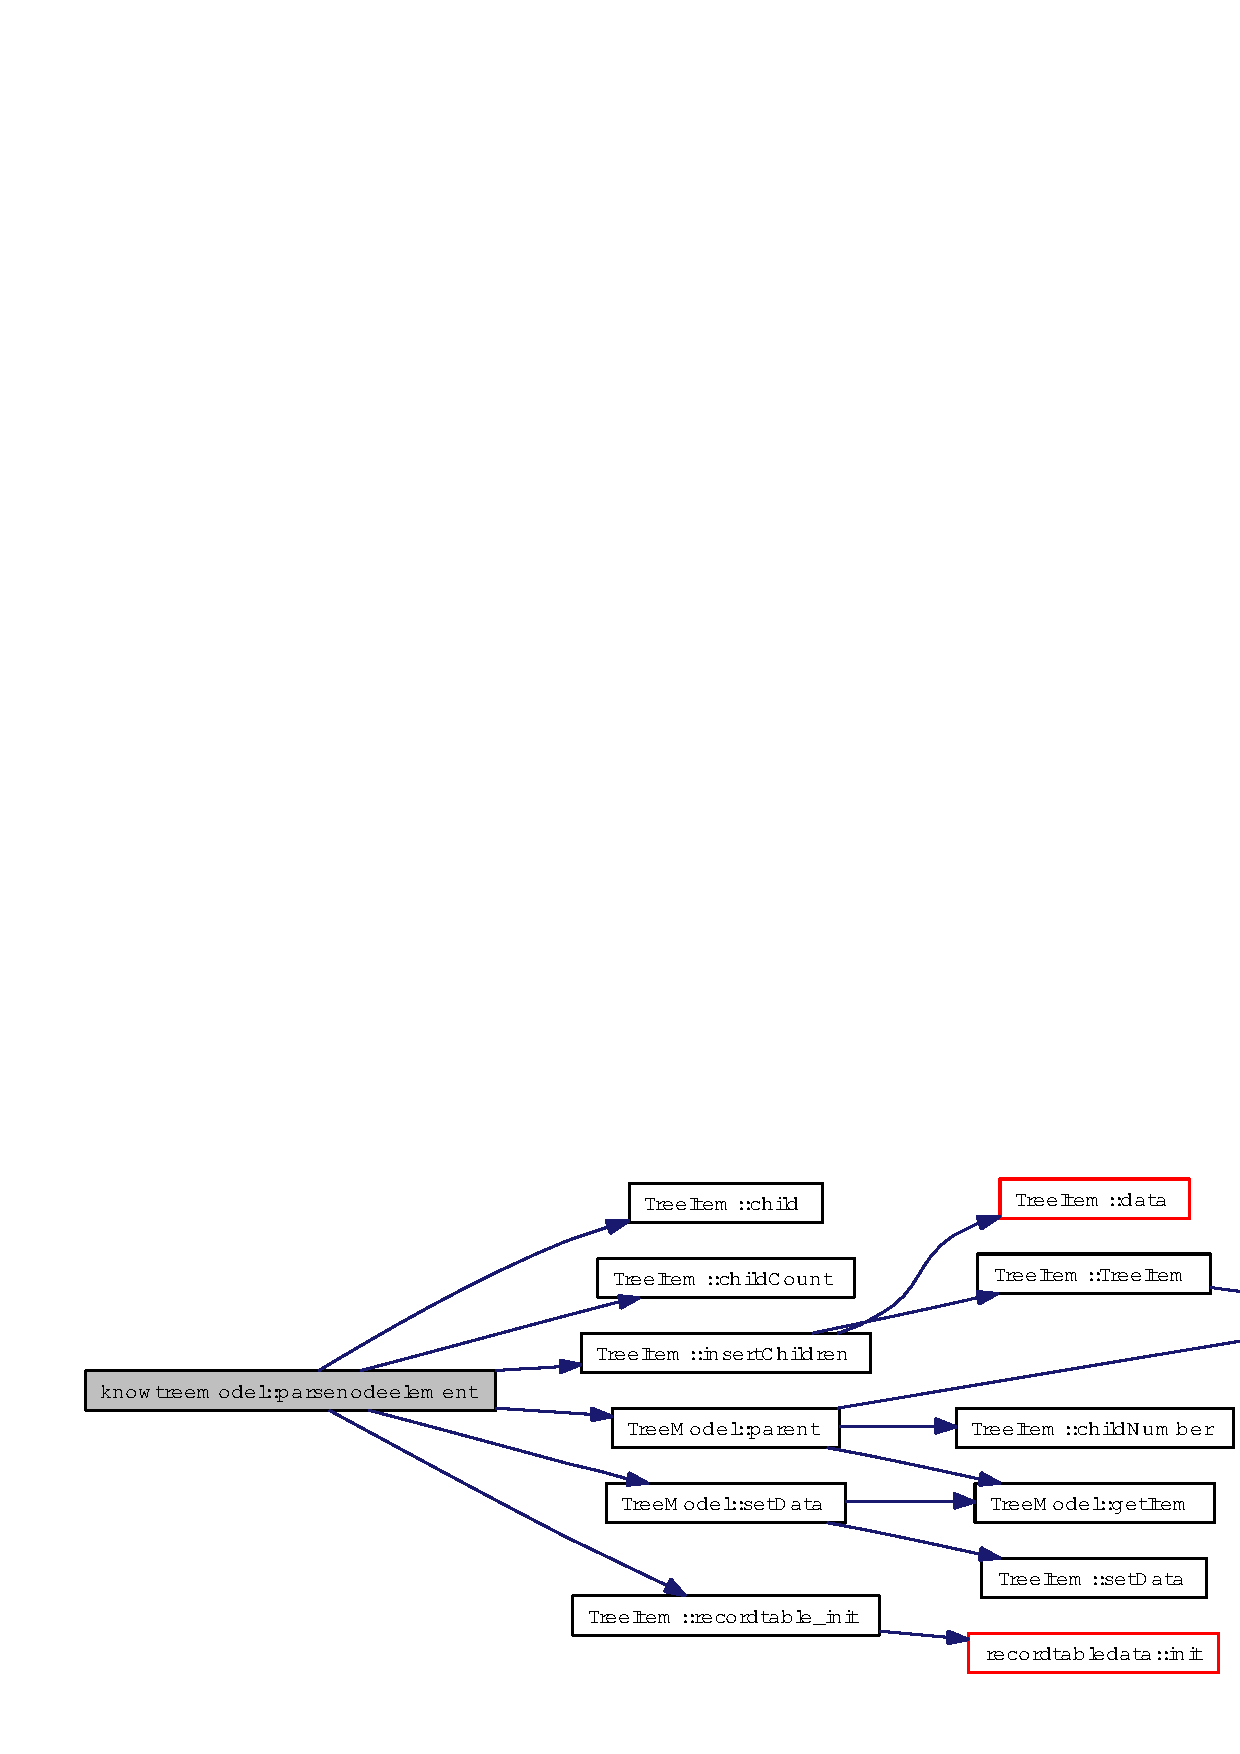
\includegraphics[width=367pt]{classknowtreemodel_01a2b1a9a1edc6b25210a27a6cca5a7c_cgraph}
\end{center}
\end{figure}


Here is the caller graph for this function:\begin{figure}[H]
\begin{center}
\leavevmode
\includegraphics[width=340pt]{classknowtreemodel_01a2b1a9a1edc6b25210a27a6cca5a7c_icgraph}
\end{center}
\end{figure}
\index{knowtreemodel@{knowtreemodel}!parsetreetodom@{parsetreetodom}}
\index{parsetreetodom@{parsetreetodom}!knowtreemodel@{knowtreemodel}}
\subsubsection{\setlength{\rightskip}{0pt plus 5cm}void knowtreemodel::parsetreetodom (QDom\-Element $\ast$ {\em xmldata}, {\bf Tree\-Item} $\ast$ {\em curritem})\hspace{0.3cm}{\tt  [private]}}\label{classknowtreemodel_f0f1bf490bdc9687d25d72b966020cd8}




Definition at line 115 of file knowtreemodel.cpp.

References Tree\-Item::child(), Tree\-Item::child\-Count(), Tree\-Item::data(), Tree\-Item::recordtable\_\-export\_\-data\_\-to\_\-dom(), and Tree\-Item::recordtable\_\-getrowcount().

Referenced by export\_\-fullmodeldata\_\-to\_\-dom().

Here is the call graph for this function:\begin{figure}[H]
\begin{center}
\leavevmode
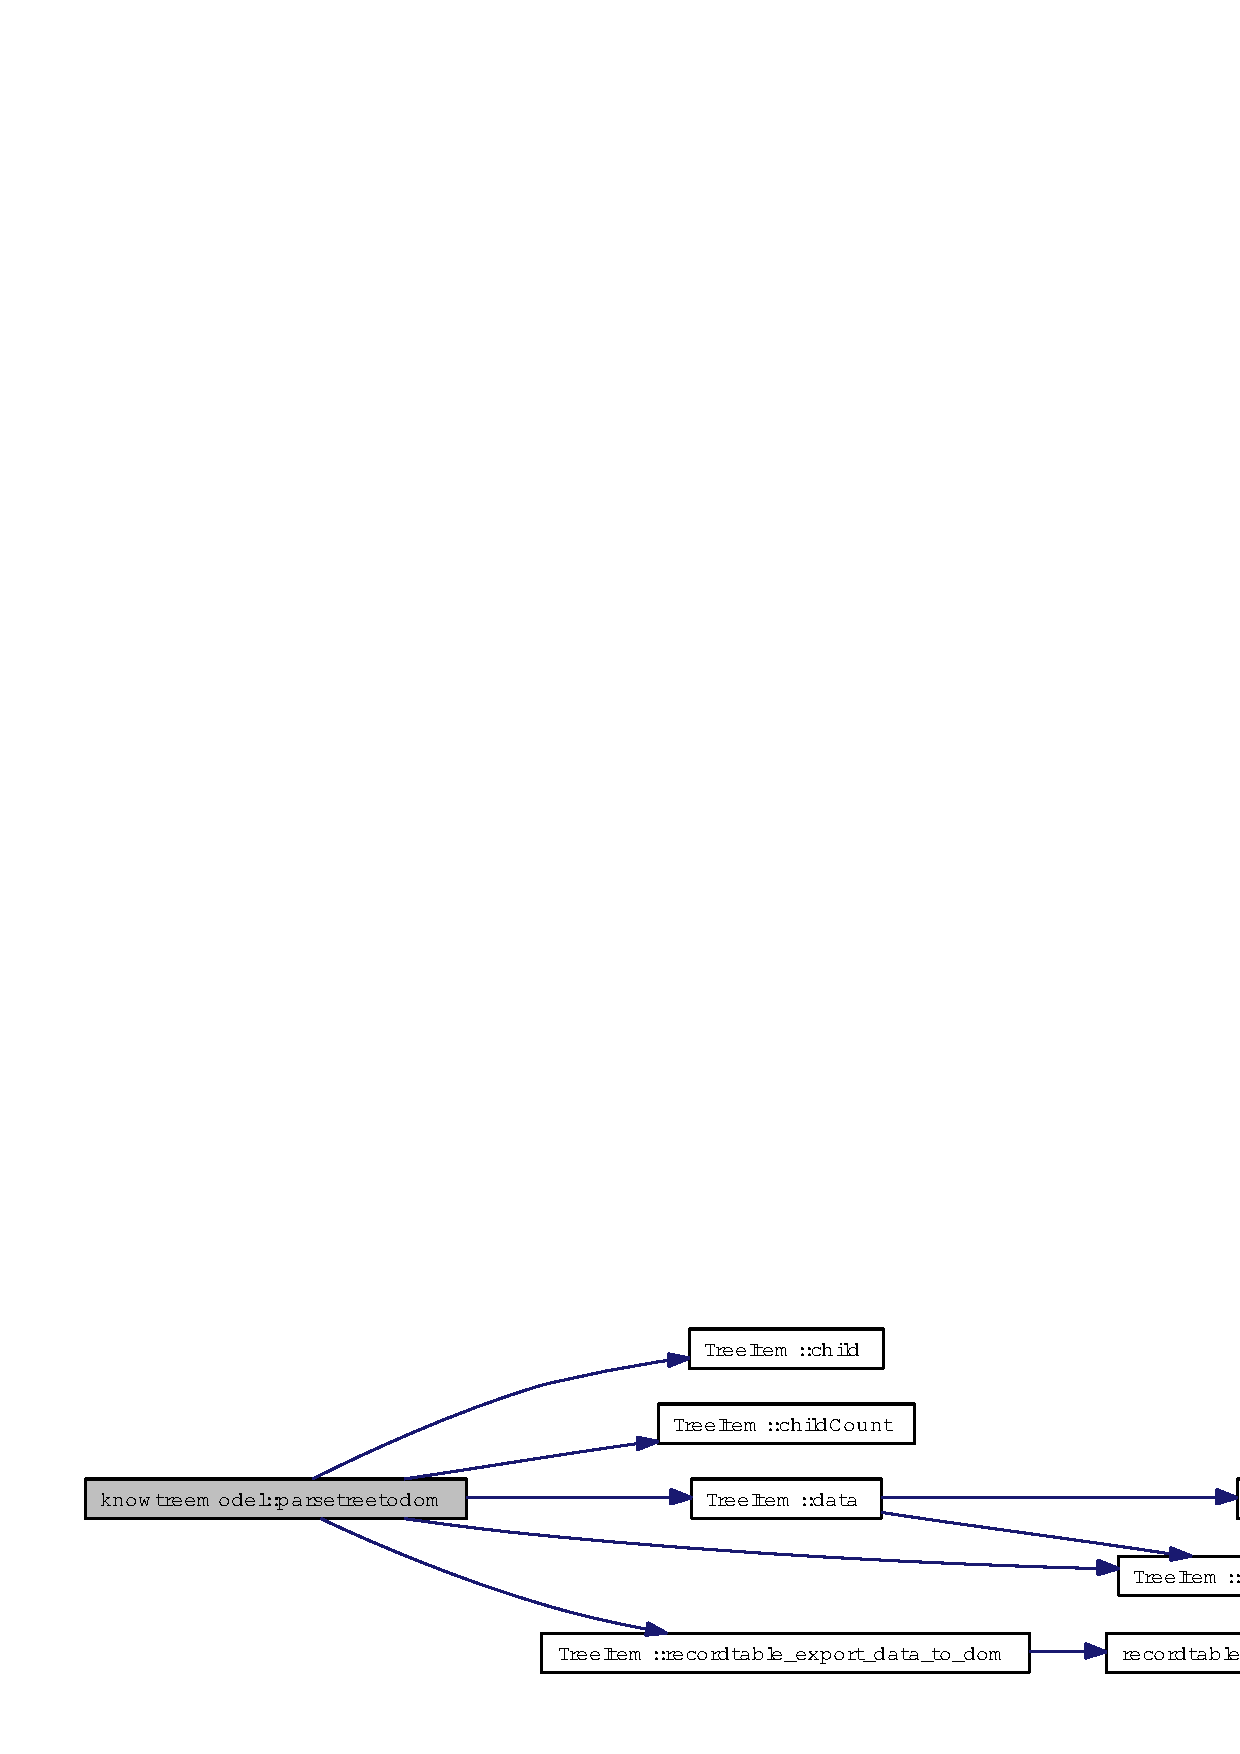
\includegraphics[width=371pt]{classknowtreemodel_f0f1bf490bdc9687d25d72b966020cd8_cgraph}
\end{center}
\end{figure}


Here is the caller graph for this function:\begin{figure}[H]
\begin{center}
\leavevmode
\includegraphics[width=354pt]{classknowtreemodel_f0f1bf490bdc9687d25d72b966020cd8_icgraph}
\end{center}
\end{figure}
\index{knowtreemodel@{knowtreemodel}!move_updn_branch@{move\_\-updn\_\-branch}}
\index{move_updn_branch@{move\_\-updn\_\-branch}!knowtreemodel@{knowtreemodel}}
\subsubsection{\setlength{\rightskip}{0pt plus 5cm}QModel\-Index knowtreemodel::move\_\-updn\_\-branch (const QModel\-Index \& {\em index}, int {\em direction})\hspace{0.3cm}{\tt  [private]}}\label{classknowtreemodel_6d0493ddfa7010baf5bd713a6f0a8a11}




Definition at line 229 of file knowtreemodel.cpp.

References Tree\-Model::get\-Item(), Tree\-Model::index(), Tree\-Item::move\_\-dn(), and Tree\-Item::move\_\-up().

Referenced by move\_\-dn\_\-branch(), and move\_\-up\_\-branch().

Here is the call graph for this function:\begin{figure}[H]
\begin{center}
\leavevmode
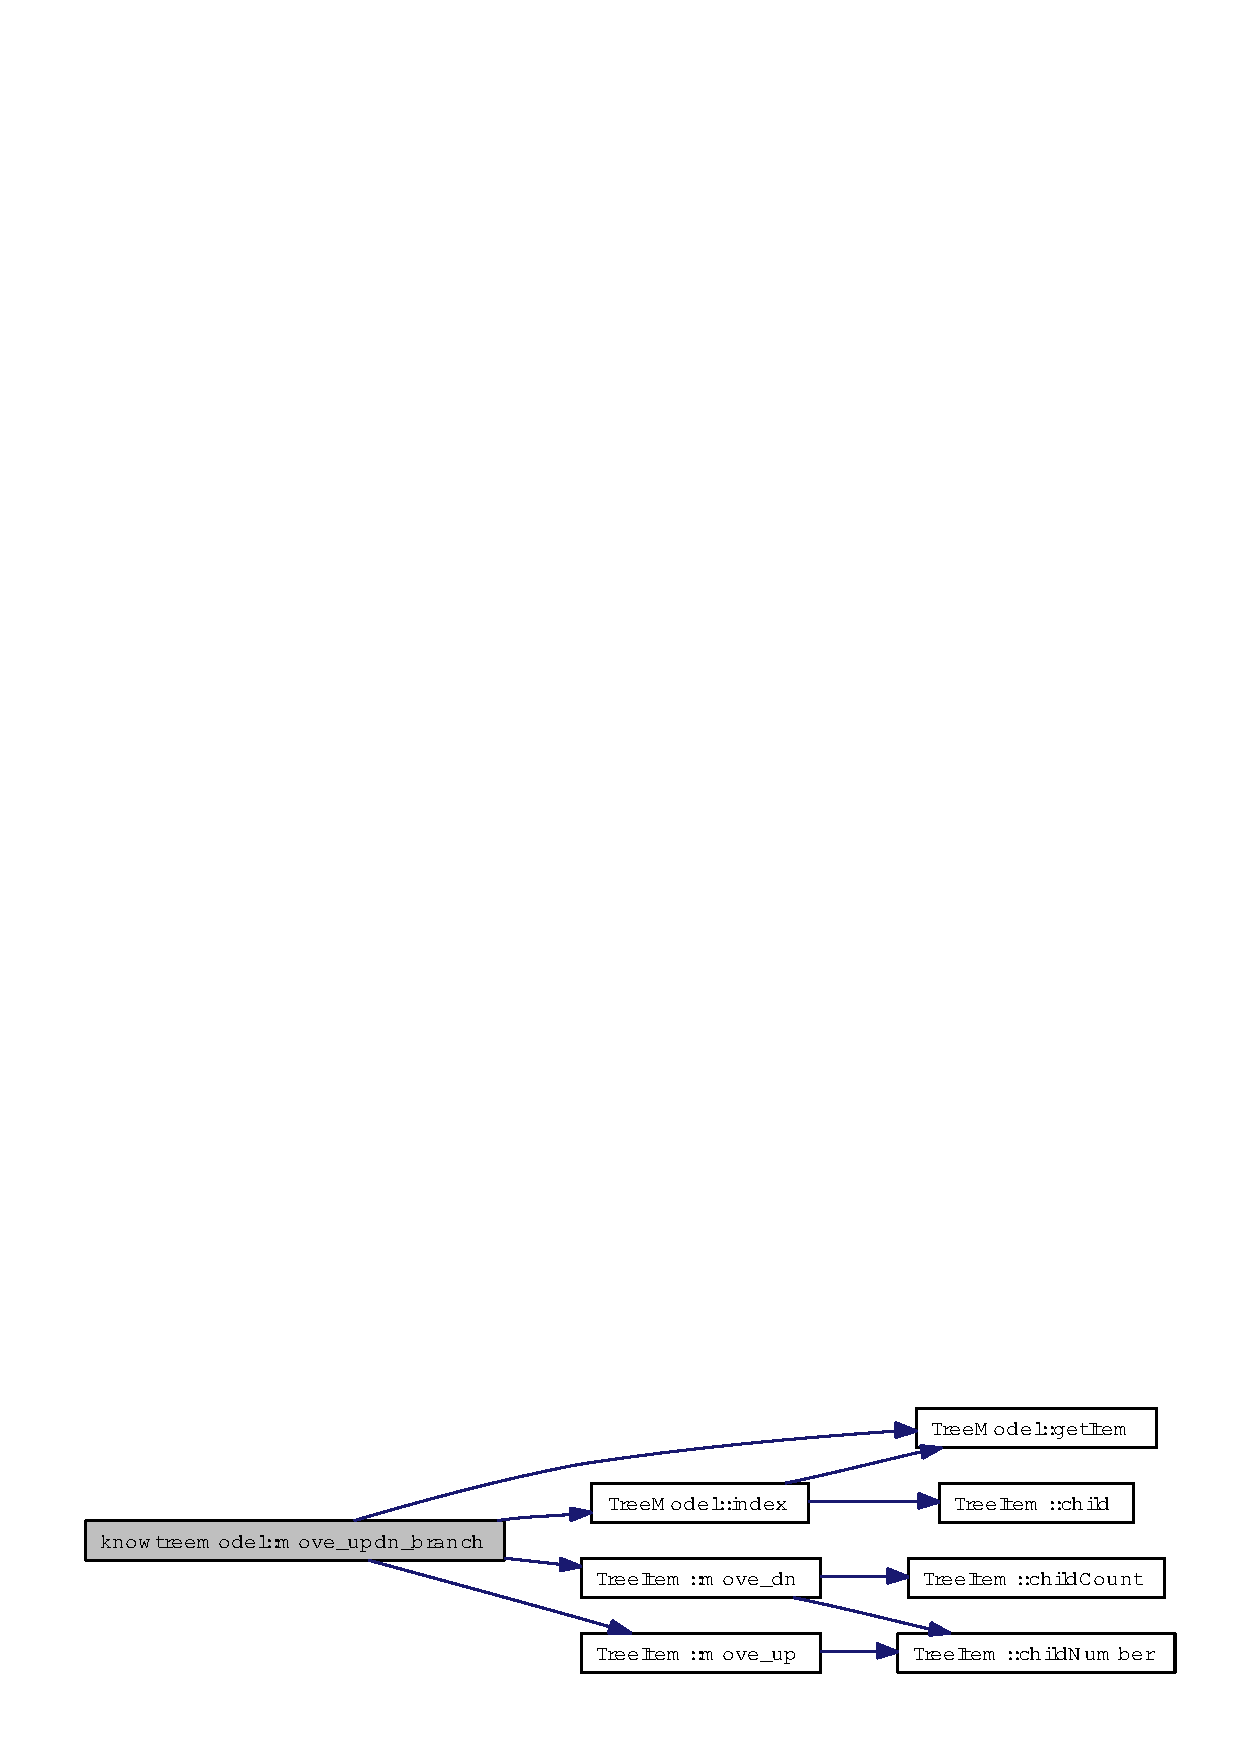
\includegraphics[width=284pt]{classknowtreemodel_6d0493ddfa7010baf5bd713a6f0a8a11_cgraph}
\end{center}
\end{figure}


Here is the caller graph for this function:\begin{figure}[H]
\begin{center}
\leavevmode
\includegraphics[width=342pt]{classknowtreemodel_6d0493ddfa7010baf5bd713a6f0a8a11_icgraph}
\end{center}
\end{figure}
\index{knowtreemodel@{knowtreemodel}!get_item_index_recurse@{get\_\-item\_\-index\_\-recurse}}
\index{get_item_index_recurse@{get\_\-item\_\-index\_\-recurse}!knowtreemodel@{knowtreemodel}}
\subsubsection{\setlength{\rightskip}{0pt plus 5cm}QModel\-Index knowtreemodel::get\_\-item\_\-index\_\-recurse (QModel\-Index {\em currindex}, {\bf Tree\-Item} $\ast$ {\em finditem}, int {\em mode})\hspace{0.3cm}{\tt  [private]}}\label{classknowtreemodel_1113f34691048a9002d8a1a1a64e1287}




The documentation for this class was generated from the following files:\begin{CompactItemize}
\item 
{\bf knowtreemodel.h}\item 
{\bf knowtreemodel.cpp}\end{CompactItemize}
